\chapter{Baseline}
\label{chap:baseline}

In this chapter, a particularly important and already existing approach for the synchronizing oscillators phases $\phi$ and frequencies $\omega$ in oscillator networks is presented. The type of synchronization, \textit{harmonic} that is, will be continued to be used in this thesis and used as the goal state also for the Dr. Squiggle system at hand. Furthermore, the baseline authors's synchronization methods will also serve as a foundation for synchronization experimentation later on, as these are implemented in the novel Dr. Squiggle synchronization simulator.

In this Active Music System, as shown in Figure \ref{fig:nymoen_fireflies_on_ios_devices}, decentralized harmonic synchronization of a dynamic and arbitrary number of musical nodes (modelled as pulse-coupled oscillators) — involving indirect coordination through stigmergy, as well as self-awareness through knowledge regarding itself internally and in publicly in the context of other nodes — is achieved.

This is done by endowing oscillators with self awareness capabilities amongst other measures, and is achieved by nodes communicating solely through audio signals. The platform Nymoen et al. achieved this on is shown in Figure \ref{fig:nymoen_fireflies_on_ios_devices}, as each firefly on their iOS devices initially start flashing unsynchronized and randomly, but then eventually manage to start firing synchronously\footnote{See video at \url{https://vimeo.com/67205605} (accessed 2022.05.17)}.

\begin{figure}[ht!]
	\centering
	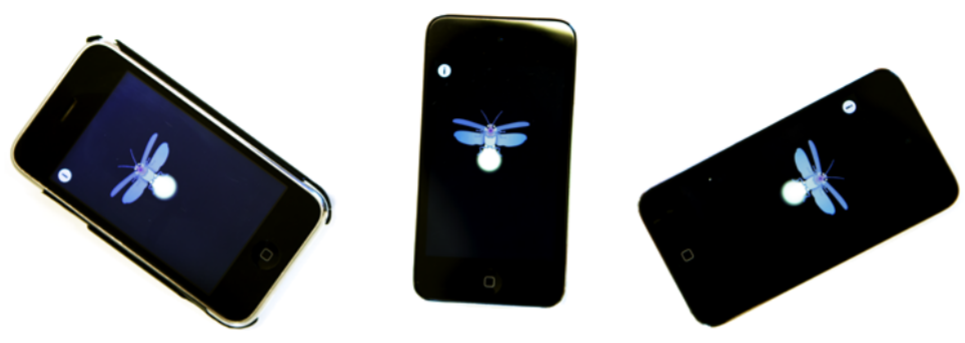
\includegraphics[width=0.7\linewidth]{Assets/DocSegments/Chapters/Baseline/Figures/Illustrations/fireflies_on_ios_devices.png}
	\caption[]{Decentralized oscillators modelled as fireflies achieving harmonic synchrony on iOS devices, after starting flashing unsynchronously. Image: K. Nymoen et al. \cite{nymoen_synch}.}
	\label{fig:nymoen_fireflies_on_ios_devices}
\end{figure}

As Nymoen designed update functions for synchronizing both phases and frequencies, not only were their firefly-inspired oscillators endowed with self awareness capabilities; they were also designed to adjust their phases and frequencies with (close to) 0 change half-way through the oscillator cycle. These (close to) 0 changes half-way through oscillators's cycles enable individual musical agents to play with different measures (e.g. half or 1/4th as fast) compared to other individuals—being characteristic for musical interaction with several musical individuals—as well as enabling the possibility of achieving the target state of harmonic synchrony (cf. \ref{sec:harmonic_synchrony}). Their contribution also differs from previous approaches in that Nymoen et al.'s fireflies only need to transmit ``fire'' signals every other phase climax, not every single phase climax; in other words, synchronization is achieved despite less communication.

First, the relatively new system target state of \textit{harmonic synchrony} will be expounded and explained in \ref{sec:harmonic_synchrony}. Then, the aforementioned update functions for both phase ($\phi$) and frequency ($\omega$), explaining the incorporated level of self awareness as well as how a decentralized collective of pulse copuled oscillators can achieve harmonic synchrony, are thus presented in \ref{sec:nymoen_phase_updates} and \ref{sec:nymoen_freq_updates}.



\section{System target state: harmonic synchrony}
\label{sec:harmonic_synchrony}

The state of harmonic synchrony is defined \cite{nymoen_synch} as the state in which all agents in the musical collective ``fire'' or ``flash'', as described in Subsection \ref{subsec:fire_signal}, at an even and underlying interval or pulse, a certain number of times in a row. This is not to say all agents will have to ``fire''/``flash'' simultaneously, as has traditionally been the case for strict synchronization in pulse-coupled oscillators. How legal and harmonically synchronized oscillator frequencies and phases look like will be described in this Section.

As one is designing and creating an interactive music technology system, one might want to encourage and allow for the playing of various musical instruments at various rhythms/paces, as it might be quite boring if all instruments were played at the exact same measure or pulse. As K. Nymoen et al. \cite{nymoen_synch} reason while discussing their own interactive ``Firefly'' music-system as well as coining the term of \textit{harmonic synchrony}: \nl

\textit{Temporal components in music tend to appear in an integer-ratio relation to each other (e.g., beats, measures, phrases, or quarter notes, 8ths, 16ths)}. \nl

and \nl

\textit{Being an interactive music system, people may want their device to synchronize with different subdivisions of a measure (e.g. some play quarter notes while others play 8ths).} \nl

Accomodating for these aspects then, K. Nymoen et al. took inspiration for coining a novel state of synchronization for a decentralized system. This novel state arose from the concept of \textit{harmonics} in the frequency spectrum of a waveform; in that each harmonic wave or overtone has a frequency with an integer relationship to the fundamental (smallest) frequency in a waveform. Such a phenomenon, used as inspiration by Nymoen et al. but not as the basis for any definitions directly, can e.g. be seen in the frequency spectrogram of a humanly hummed G3-tone, depicted in Figure \ref{fig:sub:G3_hummed_waveform}. In said example, one can observe the presence of harmonics and overtones having frequencies with integer relationships to the fundamental (smallest) frequency at around 196 Hz, as we see the overtones e.g. has frequencies of around 400Hz, 800Hz, and 1600Hz. We will soon see how such relationships in frequency are used as inpiration for a new definition of a synchronous state; however, the example in Figure \ref{fig:frequency_spectrograms} is only meant to give an idea of where this new state of synchronization stems from, and not as a visual representation of said novel synchrony state.

\begin{figure}[ht!]
	\centering
	\begin{subfigure}[t]{.5\textwidth}
		\centering\captionsetup{width=.9\linewidth}%
		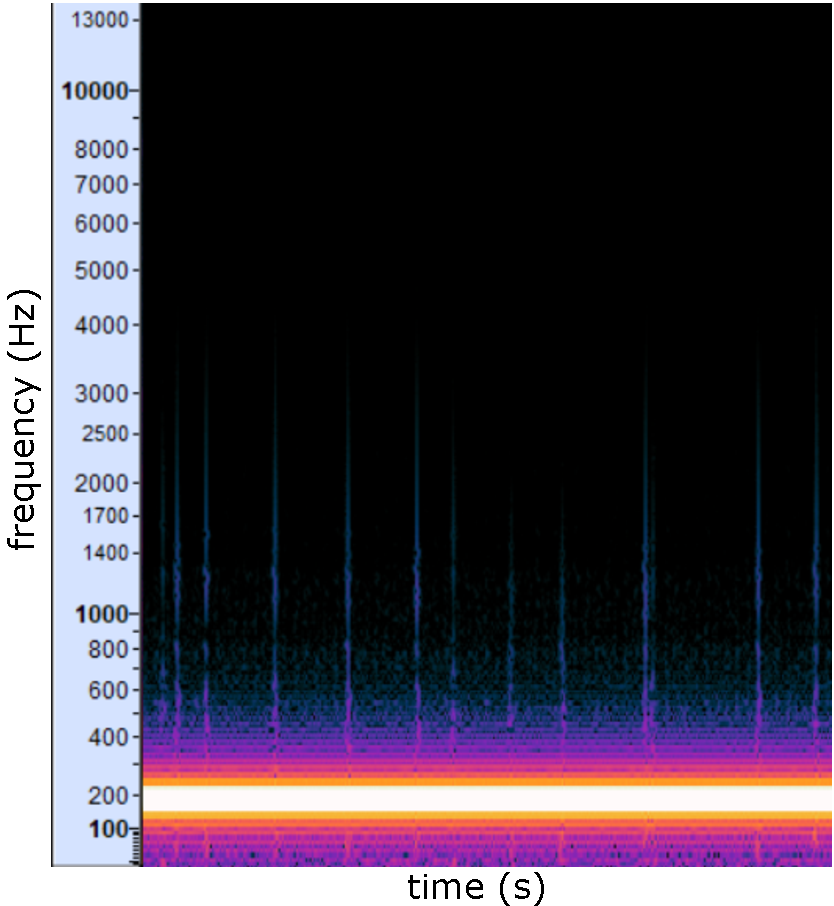
\includegraphics[width=0.9\linewidth]{Assets/DocSegments/Chapters/Baseline/Figures/Illustrations/G3_196Hz_PureTone_waveform_spectrogram.pdf}
		\caption{The frequency spectrogram of the audible waveform being a monotone and purely generated\protect\footnotemark  G3-tone at 195.99 Hz.}
		\label{fig:sub:G3_pure_waveform}
	\end{subfigure}%
	\begin{subfigure}[t]{.5\textwidth}
		\centering\captionsetup{width=.9\linewidth}%
		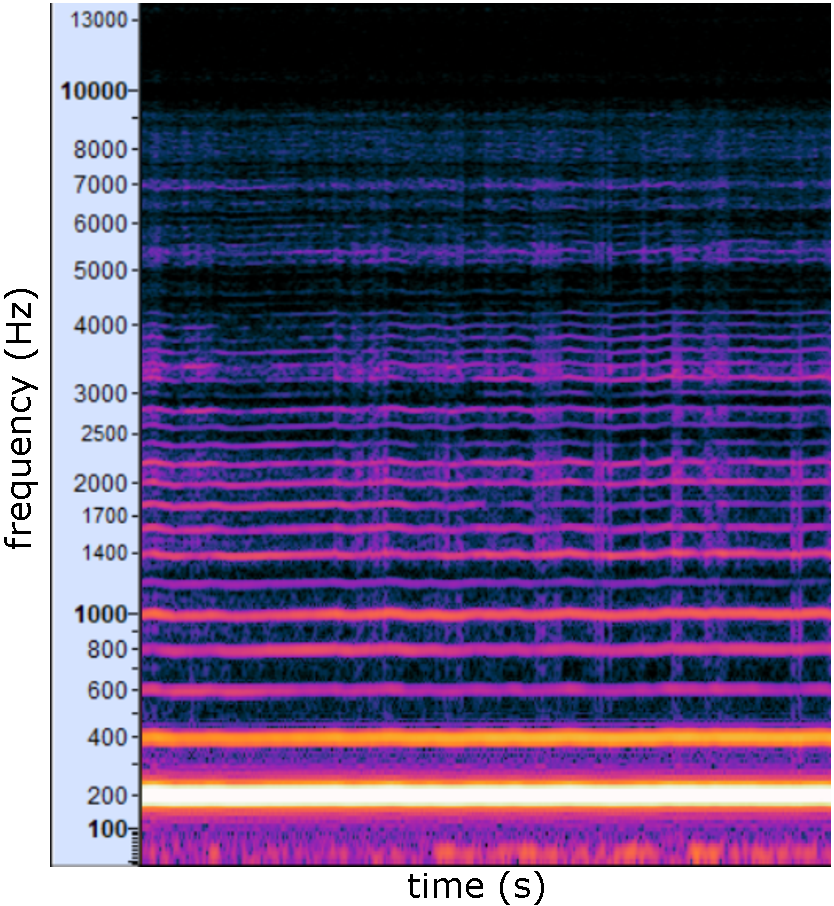
\includegraphics[width=0.9\linewidth]{Assets/DocSegments/Chapters/Baseline/Figures/Illustrations/G3_196Hz_HummingWaveform_FrequencySpectrum.pdf}
		\caption{The frequency spectrogram of the audible waveform being a more-or-less monotone but non-pure G3-tone, hummed and recorded\protect\footnotemark  by me, as I tried to repeat the tone in \ref{fig:sub:G3_pure_waveform} with my voice.}
		\label{fig:sub:G3_hummed_waveform}
	\end{subfigure}
	\caption[Frequency spectrograms illustrating the absence and presence of harmonics and overtones in audible waveforms.]{Frequency spectrograms of two different-sounding waveforms of the same G3-tone at 195.99 Hz. Note the absence and presence of harmonics and overtones in waveform \ref{fig:sub:G3_pure_waveform} and \ref{fig:sub:G3_hummed_waveform} respectively, as well as the integer-relationships between the fundamental (lowest) frequency and the harmonics in \ref{fig:sub:G3_hummed_waveform}. Frequencies in a harmonically synchronized oscillator collective will for the first phase synchronization problem resemble the frequencies in \ref{fig:sub:G3_pure_waveform}, where all frequencies are equal and constant. Conversely, when frequencies can initially be heterogenous and unequal, as in the phase \textit{and} frequency synchronization problem, the frequencies in a harmonically synchronized oscillator collective will rather resemble, although not completely correspond to, the frequencies in \ref{fig:sub:G3_hummed_waveform}, where higher frequencies with integer relationships to the fundamental and lowest frequency can be present at the same time.}
	\label{fig:frequency_spectrograms}
\end{figure}

\addtocounter{footnote}{-2} %2=n
 \stepcounter{footnote}\footnotetext{\url{https://www.szynalski.com/tone-generator/} (accessed 2022.05.17)}
 \stepcounter{footnote}\footnotetext{\url{https://github.com/theRealSherapat/CompSA/blob/main/CollectedData/Audio/G3_196Hz_humming.wav} (accessed 2022.05.22)}


More accurately then and inspired by integer relationships in waveforms, although not exactly analogus to the example above in Figure \ref{fig:frequency_spectrograms}, Nymoen et al. describe \textit{legal} frequencies the oscillator frequencies has to lie within to be considered \textit{harmonically synchronized}. Frequencies have to lie within 

\begin{equation}\label{nymoen_legal_freqs}
\omega_{0} \cdot 2^{\mathbb{N}_0}, 
\end{equation}

where $\omega_0$ represents the smallest oscillator frequency in the oscillator collective, and $\mathbb{N}_0$ are the natural numbers including the number zero.

Note that the only difference between Nymoen's definition of \textit{legal oscillator frequencies} and the spectrogram example depicted in Figure \ref{fig:frequency_spectrograms} lies in that for the legal frequencies as defined in \eqref{nymoen_legal_freqs}, higher frequencies can only have doubling integer relationships with the lowest fundamendal frequency (e.g. twice or four times as high), whereas the frequencies of the harmonics seen in the humanly hummed G3 tone (\ref{fig:sub:G3_hummed_waveform}) additionally had all other positive integer relationships (e.g. three or five times as high) with the fundamental frequency.

	\subsection{Detecting harmonic synchrony}
	\label{baseline:subsec:detecting_harmonic_sync}
	In order to test and evaluate synchronization performance in their firefly-inspired oscillator-system, K. Nymoen et al. \cite{nymoen_synch} develop a measurement used to detect when the system has reached a state of synchrony. Using the firings of the fireflies, some key and well-defined conditions have to be met in order for the fireflies to be deemed \textit{harmonically synchronized}: \nl
	
	\textbf{Harmonic synchronizaton conditions:}
	
	\begin{itemize}
		\item[] \textbf{Condition 5)}: Firing may only happen within a short time period $t_f$.
		\item[] \textbf{Condition 6)}: Between each $t_f$, a period $t_q$ without fire events must be equally long $k$ times in a row.
		\item[] \textbf{Condition 7)}: All nodes must have fired at least once during the evaluation period.
	\end{itemize}
	\sep
	
	Visually, these requirements are shown in Nymoen's sketch for detecting harmonic synchrony in Figure \ref{fig:nymoen_harm_sync_detect}.
	
	\begin{figure}[ht!]
		\centering
		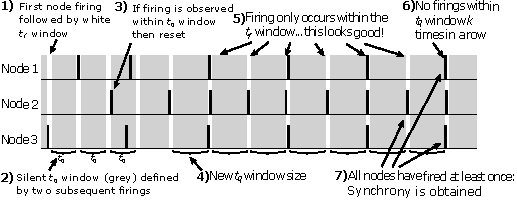
\includegraphics[width=\linewidth]{Assets/DocSegments/Chapters/Baseline/Figures/Illustrations/NymoenHarmonicSyncDetectionSchema.pdf}
		\caption[Nymoen et al.'s harmonic synchrony detection schema.]{Requirements needing to be fulfilled in order to have achieved the target state of harmonic synchrony in an oscillator (here meant by ``node'') collective. Image: K. Nymoen et al. \cite{nymoen_synch}.}
		\label{fig:nymoen_harm_sync_detect}
	\end{figure}
	
	Steps \textbf{1) - 4)} are means to achieve \textbf{5) - 7)}.
	
	In summary, by utilizing transmitted firings or pulses from the robots in our robot collective, the aforementioned harmonic synchrony conditions can be enforced and checked throughout the synchronization process, in order to detect if, and in that case when, the oscillator network becomes harmonically synchronized. The time having passed from the start of the synchronization-process until the detection of harmonic synchrony will then be defined as the performance score, indicating how fast or slow the oscillators are at synchronizing.
	
	These harmonic synchrony requirements, as well as Nymoen's schema in Figure \ref{fig:nymoen_harm_sync_detect}, thus constitutes a blueprint for the design of a performance or synchrony measure able to detect the achievement of harmonic synchrony in a decentralized network of pulse coupled oscillators ``firing'' pulses in order to synchronize to each other; which is exactly what's implemented in this thesis's synchronization system to be explained further in Chapter \ref{chap:implementation}.
	
	% The exact details of how such a performance / synchrony measure is implemented for the synchronization system in this thesis will be given in Section \ref{sec:detecting_harmonic_synchrony} in Chapter \ref{chap:implementation}.
	
% —- \section END. —-



\section{Phase synchronization} % or adjustment
\label{sec:nymoen_phase_updates}

	In their firefly system, synchronization of the phase values $\phi$, representing where the oscillator are in their cycles (e.g. in the start or end of its period), is achieved. By utilizing bi-directional phase shifts, oscillators depending on being in the first or second half of its phase cycle, i.e. $\phi < 0.5$ or $\phi > 0.5$, adjust their phases by either subtracting from the phase, or adding to it. This they do based on their phase update function, $P(\phi)$, as shown in \eqref{nymoen_phase}.

	\subsection{Problem statement}

	In this first and more simple synchronization problem, which we call the \textbf{phase ($\phi$) synchronization problem}, we assume homogenous and already-synchronized frequencies $\omega_i=1Hz$ for all oscillators $i$. The oscillator collective hence only has to synchronize phases $\phi_i$ for all oscillators $i$, which are initially uniformly random phase values $\in [0,1]$. Hence, phase adjustments are needed in order to synchronize phases in the pulse coupled oscillator collective.

	
	\subsection{Synchronizing phases via phase adjustment}

	\textbf{K. Nymoen's bi-directional phase adjustment} \nl % or 'shifts', as used before.
	\label{subsec:nymoen_phase_adjust}

	Apart from altering a similar phase adjustment function to the likes of Mirollo-Strogatz's phase adjustment function \eqref{strog_phase} sketched in Figure \ref{fig:mirollo_strogatz_phase_adj_sketch}, K. Nymoen et al. \cite{nymoen_synch} introduces an example of a bi directional phase adjustment method. This they do mainly so that their phase adjustment ($Adj_{\phi}$) method would cooperate well with their system's frequency adjustment, in order to achieving their target goal of harmonic synchrony. The difference between a bi directional method of phase synchronization and a one directional one is that using bi directional phase adjustment, oscillators are simply adjusting each other's phases in an excitatory way; they only ``push'' other ocillators's phases further or higher (positive updates) when firing themselves, never ``holding'' or ``dragging'' them back (negative updates).

	Hence, this newer approach to phase adjustment works very similarly to the phase adjustment performed in the ``standard'' \textbf{\textit{Mirollo-Strogatz}} approach presented earlier; the only difference being that now, oscillators update their phases with the slightly more complex \textbf{phase update function \eqref{nymoen_phase}} when hearing a ``fire''-event from one of the other musical nodes — allowing for both larger, but also smaller, updated phases compared to the old phases:

	\begin{equation}
	\label{nymoen_phase}
		\phi(t^+)=P(\phi(t)) = \phi(t) - \alpha \cdot sin(2\pi\phi(t)) \cdot | sin(2\pi\phi(t)) | ,
	\end{equation} \nl
	where $t^+$ denotes the time-step immediately after a ``fire''-event is heard, and $\phi(t)$ is the old frequency of the oscillator at time $t$.

	The fact that new and updated phases can both be larger, but also smaller, compared to the old phases, is exactly what's meant by the phase-adjustment being \textbf{\textit{bi-directional}}, or as the authors call it in the paper as using both excitatory and inhibitory phase couplings between oscillators \cite{nymoen_synch}.

	The effects then of adjusting phases—upon hearing ``fire''-events, according to this newest update-function \eqref{nymoen_phase}—are that the nodes's updated phases $\phi(t^+)$, compared to their old phases $\phi(t)$, now get decreased if $\phi(t)$ is lower than 0.5, increased if $\phi(t)$ is higher than 0.5, and neither—at least almost—if the phases are close to $0.5$. This is due to the negative and positive sign of the sinewave-component in Equation \eqref{nymoen_phase}, as well as the last attenuating factor in it of $| sin(2\pi\phi) | \approx | sin(2\pi \frac{1}{2}) | = | sin(\pi) | = | 0 | = 0$, then if we have $\phi(t) \approx 0.5 = \frac{1}{2}$.

% —- \section END. —-



\section{Phase and frequency synchronization}
\label{sec:nymoen_freq_updates}

	Nymoen also achieved synchronizing the frequency values $\omega$ of oscillators, being the speed at which the oscillator cycles through its cycle or oscillator period at (cf. \eqref{phase_freq}).
	
	This they managed to do by as mentioned and amongst other measures implementing an aspect of \textit{self awareness} in terms of a \textit{synchrony self assessment} $s(n)$ given ``fire'' event $n$, representing how much or out of sync an individual robot is.
	
	It will then, having taken into account some middle steps as explained below, use this self assessed sync score $s(n)$ to obtain a frequency adjustment contribution $H(n)$ for ``fire'' event $n$, which will tell in what direction and how much the frequency should be adjusted. As many such $H(n)$ values will be calculated and accumulated in a firefly as said firefly hears fire events throughout its oscillator period / cycle—before they are used for frequency updating at the end of the cycle. This way of performing frequency updates are inspired by Werner-Allen's reachback firefly algorithm (RFA), simply meaning updates are postponed until the end of the cycle instead of happening immediately as a fire event is received.
	
	Now the system used for comparison later on in the synchronization simulator is explained further in detail.
	

	\subsection{Problem statement}

	In this second and more challenging synchronization problem, which we call the \textbf{phase and frequency ($\phi \& \omega$) synchronization problem}, we no longer assume homogenous and already-synchronized oscillator frequencies like in the first phase ($\phi$) synchronization problem when all frequencies were fixed to 1Hz. Now, the oscillators's frequencies are initialized to uniformly random frequencies $\omega_i$ within a certain minimum initial frequency $\omega_{min}^{init}$ (e.g. 0.5Hz) and maximum initial frequency $\omega_{max}^{init}$ (e.g. 4Hz).
	Hence, the problem is now more complex; the oscillator collective not only has to synchronize all initially random phases $\phi_i$ as above, but simultaneously, also all initially random frequencies $\omega_i$ for all oscillators $i$ as well. Hence, both phase \textit{and} frequency adjustments are needed in order to synchronize both phases $\phi$ and frequencies $\omega$ in the oscillator collective.


	\subsection{Synchronizing frequencies via frequency adjustment}
	\label{subsec:nymoen_freq_adj}

	Only one frequency adjustment / update function was used as a starting point for this thesis and eventually implemented in the Unity synchrony simulator. This one frequency synchronization method, as invented by Nymoen et al. \cite{nymoen_synch}, is now presented. \nl

	\textbf{K. Nymoen's frequency adjustment} \nl
	This approach to frequency adjustment in pulse coupled oscillators, in order to achieve synchronized frequencies, stands in contrast to previous approaches of synchronization where oscillators frequencies are either equal and fixed, oscillators have to send out a pulse every oscillator cycle, or they do not include any explicit self awareness capabilities. This is not the case for Nymoen's frequency adjustment.

	In order to achieve \textit{harmonically synchronized} and ``legal'' oscillator frequencies (cf. \ref{sec:harmonic_synchrony}) in the oscillator collective, not only the phases ($\phi$) have to be adjusted and eventually synchronized; frequencies ($\omega$) also have to be synchronized through frequency adjustment.
	
	\begin{figure}[ht!]
		\centering
		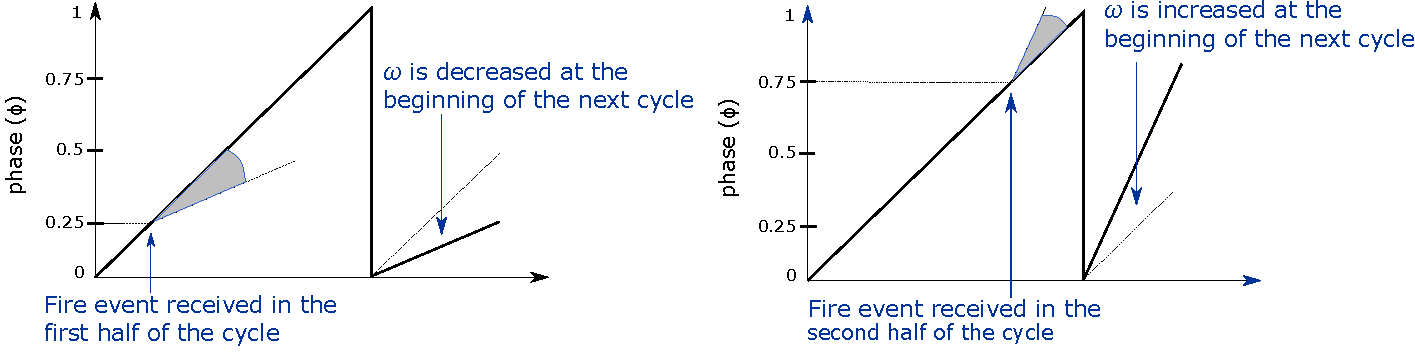
\includegraphics[width=\linewidth]{Assets/DocSegments/Chapters/Baseline/Figures/Illustrations/NymoenFrequencyAdjustment.pdf}
		\caption[]{An illustration of how frequencies are adjusted after each phase climax (i.e. $\phi=1$) using Nymoen et al.'s frequency update function. Reproduced from \cite{nymoen_synch}.}
		\label{fig:nymoen_freq_adjust_illustration}
	\end{figure}
	
	When it comes to the temporality and timing of when these update functions are used and applied; Musical agents's phases get updated/adjusted immediately as ``fire'' events are perceived, whereas agents's frequencies do not get updated until the end of their oscillator-cycle (i.e. when having a phase-climax $\phi(t)=1$). This is also the reason why frequencies are updated discretely, not continuously. So-called H-values however, being ``contributions'' with which the frequencies are to be updated according to, are immediately calculated and accumulated when agents are perceiving a ``fire'' event — and then finally used for frequency-adjustment/-updating at phase-climaxes.
	
	Each oscillator $i$ updates their frequency, on their own phase-climax (i.e. when $\phi_i(t)=1$), according to the frequency-update function $\omega_i(t^+)$:

	\begin{equation}
		\omega_i(t^+) = \omega_i(t) \cdot 2^{F(n)},
	\end{equation}

	where $t^+$ denotes the time-step immediately after phase-climax, $\omega_i(t)$ is the old frequency of the oscillator at time $t$, and $F(n) \in [-1,1]$ is a quantity denoting how much and in which direction an oscillator should update its frequency after having received its $n$th ``fire''-signal.

	The following steps is how the aforementioned $F(n)$ value is found: 
	
	%, and can also be refound in Algorithm \ref{AddNthFireEventsHToList} and \ref{RFAAdjustFrequency} in Chapter \ref{chap:implementation}:

		\paragraph{Step 1: $\epsilon$, the ``in-/out-of synch'' error measurement score \nl}

		Describing the error measurements at the n-th ``fire''-event, we introduce an error measurement function.

		The error measurement function value \eqref{error_measurement} is calculated immediately by each oscillator $i$, having phase $\phi_i(t)$, when a ``fire'' event signal from another oscillator $j, j \neq i$ is detected by oscillator $i$ at time $t$.

		\begin{equation}
		\label{error_measurement}
			\epsilon(\phi_i(t)) = sin^2(\pi\phi_i(t))
		\end{equation} \nl
		
		% DROPPE?
		% \begin{figure}[ht!]
			% \centering
			% 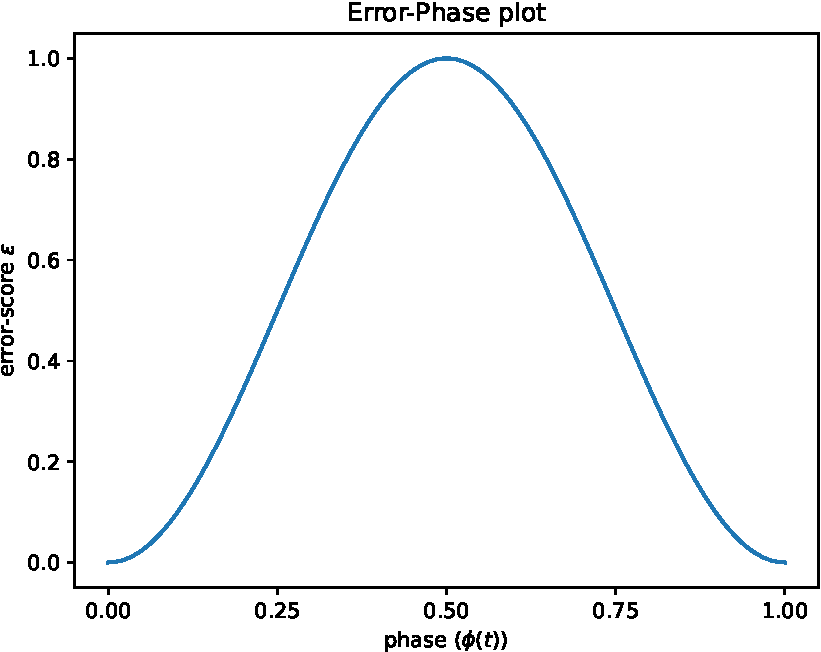
\includegraphics[width=0.65\linewidth]{Assets/DocSegments/Chapters/Baseline/Figures/Functions/PhaseErrorFunction.pdf}
			% \caption[Plot of error-measurement function for K. Nymoen's frequency-adjustment]{Error measurement \eqref{error_measurement} plotted as a function of phase}
			% \label{fig:error_measurement}
		% \end{figure}

		As we can see from this error-function, the error-score is close to 0 when the oscillator phase $\phi_i(t)$ is itself close to 0 or 1 (i.e. the oscillator either just fired/flashed, or is about to fire/flash very soon). This implies that if it was only short time ago since we just fired, or conversely if there is only short time left until we will fire, we are not much in error or \textit{out-of-synch}. 

		The error-score is the largest when an oscillator perceives a ``fire''-signal while being half-way through its own phase (i.e. having phase $\phi(t)=0.5$). We could also then ask ourselves, does not this go against the main/target goal of the system, being \textit{harmonic synchrony} — if agents are allowed to be ``half as fast'' as each other? We could imagine a completely ``legal'' and harmonically synchronous scenario where two agents have half and double the frequency of each other. The oscillator with half the frequency of the faster oscillator would then have phase $\phi(t)=0.5$ when it would hear the faster oscillator ``fire''/``flash'' — leading to its error score $\epsilon(0.5) = sin^2(\pi/2) = 1$, which then makes it seem like the slower oscillator is maximally out of synch, when it is actually perfectly and harmonically synchronized. This calls out for an attenuating mechanism in our frequency update function, in order to ``cancel out'' this contribution so that perfectly harmonically synchronized agents will not be adjusted further despite their high Error-measurement. As we will see below, exactly such an attenuating mechanism is utilized in our frequency-adjustment method.

		This error-measurement/-score forms the basis and fundament for the first component of self-awareness, being the \textit{self-assessed synchrony-score} $s(n)$.


		\paragraph{Step 2: $s$, the self-awareness component \nl}
		\label{s_n}
		This aforementioned self-assessed synchrony-score, $s(n)$, is in fact simply the median of error-scores $\epsilon$.

		If we then have a high $s(n)$-score, it tells us that the median of the $k$ last error-scores is high, or in other words that we have mainly high error-scores — indicating that this oscillator is out of synch. Conversely, if we have a low $s(n)$-score, indicating mainly low error-scores for the oscillator — then we have an indication that the oscillator is in synch, hence leading to low error scores, and in turn low $s(n)$-scores. 

		In other words, each oscillator hence has a way to assess themselves in how much in- or out-of-synch they believe they are compared to the rest of the agents. This is then the first level of self-awareness in the design.

		\paragraph{Step 3: $\rho$, the frequency update amplitude \& sign factor \nl}

		Describing the amplitude and sign of the frequency-modification of the n-th ``fire-event'' received. It is used to say something about in which direction, and in how much, the frequency should be adjusted.

		\begin{equation}
		\label{amp_sign_freq_adj}
			\rho(\phi) = - sin(2\pi\phi(t)) \in [-1, 1]
		\end{equation}

		% DROPPE?
		% \begin{figure}[ht!]
			% \centering
			% 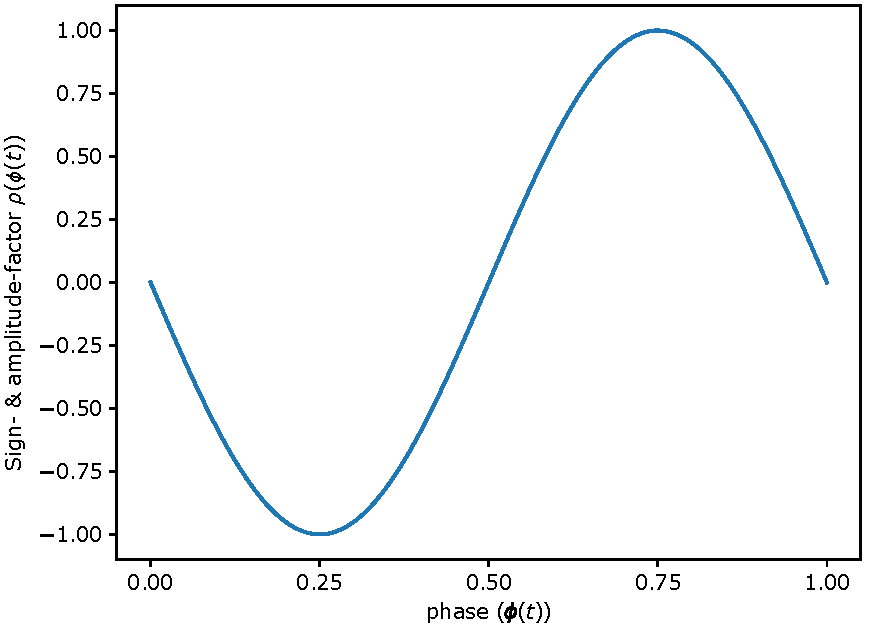
\includegraphics[width=0.65\linewidth]{Assets/DocSegments/Chapters/Baseline/Figures/Functions/rho_n.pdf}
			% \caption[Plot of amplitude- \& sign-factor for K. Nymoen's frequency-adjustment]{The amplitude- \& sign-factor, $\rho(\phi(t))$, where $\phi(t)$ is the phase of an oscillator at time $t$ when it heard ``fire''-event $n$. Notice how the amplitude is equal to 0 when the phase is equal to 0,5.}
			% \label{fig:rho_n}
		% \end{figure}

		For example, if an oscillator $i$ has phase $\phi_i(t)=1/4$, it gets a value $\rho(1/4) = - sin(\pi/2) = -1$; meaning, the oscillator's frequency should be decreased (with the highest amplitude actually) in order to "slow down" to wait for the other nodes. Conversely, if an oscillator $j$ has phase $\phi_j(t)=3/4$, it gets a value $\rho(3/4) = - sin(3/2 \pi) = -(-1) = 1$; meaning, the oscillator's frequency should be increased (with the highest amplitude) in order to getting "pushed forward" to catch up with the other nodes.

		Acts as an attenuating factor, when $\phi(t)\approx0.5$, in the making of the H-value — supporting the goal of \textit{harmonic synchrony}.
		

		\paragraph{Step 4: $H$, the frequency update contribution \nl}
		\label{H_n}

		The following value, acting as ``frequency update contributions'', is then as previously mentioned calculated immediately after the oscillator perceives another oscillator's ``flashing'' signal:

		\begin{equation}
		\label{h_value}
			H = \rho \cdot s
		\end{equation}

		Here we then multiply the factor $\rho(n)$ representing how much, as well as in which direction, the oscillator should adjust its frequency, together with a factor $s \in [0,1]$ of the adjusting oscillator's self-assessed synch-score. This implies that $H \in [0, \rho(n)$]. We hence see that the smallest value $H(n)$ can take for the $n$th ``fire''-event is -1, which it does when $\phi = 0.25$ and $s = 1$. The highest value it can take is 1, which it does when $\phi = 0.75$ and $s = 1$. We can also see that even though the self-assessed synch-score $s(n)$ (i.e. the median of error-scores) is high and even the maximum value of 1, thus indicating consistent high error-scores (judging by error-function \eqref{error_measurement}) — the ``frequency-update-contribution'' $H(n)$ can in the end be cancelled out, as alluded to before, if in fact the amplitude- \& sign-factor $\rho(n)$ is equal to 0. Hence, if we have two agents then where the one is twice as fast as the other, and we accept the $H(n)$-value as the ``frequency-update-contribution'', the slower oscillator which will hear ``fire''-events consistently when it has its phase $\phi \approx 0.5$ (if the agents are synchronized) will, even though it gets a high \textit{out-of-synch score} $s \approx 1$, not ``be told'' to adjust its frequency more by getting a large ``frequency-update-contribution'', but in fact ``be told'' not to adjust its frequency more due to the small or cancelled-out ``frequency-update-contribution.''

		% DROPPE?
		% \begin{figure}[ht!]
			% \centering
			% 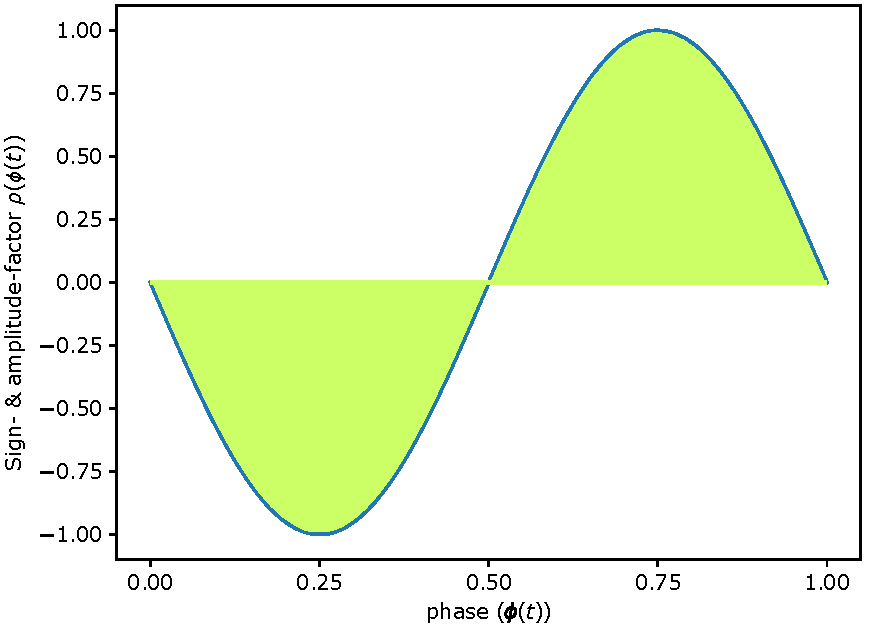
\includegraphics[width=0.65\linewidth]{Assets/DocSegments/Chapters/Baseline/Figures/Functions/all_possible_H_n_values.pdf}
			% \caption[Plot of all possible frequency-adjustment contribution-values, $H(n)$-values, for K. Nymoen's frequency-adjustment]{All possible $H(n)$-values marked in green, given by $\rho \cdot s(n)$, where $\rho(n)$ is defined as above and depicted in Figure \ref{fig:rho_n}, and the self-assessed synch-scores $s \in [0, 1]$. The $s(n)$-scores were again simply the median of $m$ error-scores \{$\epsilon(n)$, $\epsilon(n-1)$, $\epsilon(n-2)$, ... , $\epsilon(n-m)$\} which again were given by the error-function \eqref{error_measurement} plotted in Figure \ref{fig:error_measurement}. Observe, in conjunction with Equation \eqref{freq_adj}, what the authors \cite{nymoen_synch} point out when describing their frequency update function, when saying that they specify a function that decreases frequency if a fire event is received in the first half of a node's cycle (i.e. phase $\phi(t)<0.5$), and speeds up if in the last half (to ``catch up' with the firing node). Also note how the wanted design of the authors, of causing (close to) 0 change to the frequency half-way through the cycle, is enabled by how the ``frequency-adjustment-contribution'' $H(n)$ can be equal to 0 despite the reacting node having high error scores and a high $s(n)$-score.}
			% \label{fig:all_possible_H_n_values}
		% \end{figure}

		To recall, the self-assessed synch-score $s(n)$ tells an adjusting oscillator how in- or out-of-synch it was during the last $m$ perceived ``fire'' events — where $s(n)=0$ signifies a mean of 0 in error-scores, and $s(n)=1$ signifies a mean of 1 in error-scores. So then if this $H$-value is to be used to adjust the nodes's frequencies with, the frequency will then be adjusted in a certain direction and amount (specified by $\rho(n)$) — given that the oscillator is \textit{enough} ``out of synch''/``unsynchronized'' (in the case $s(n)$ is considerably larger than 0).

		The H-value says something about how much out of phase the oscillator was at the time the oscillator's $n$th ``flashing''-signal was perceived (and then followingly how much it should be adjusted, as well as in which direction after having been multiplied together with a sign-factor $\rho(n))$, given then that this H-value also consists of the \textit{self-assessed synch score s(n)} — which again simply was the median of error-scores.

		We could look at this $H$-value as representing the direction and amplitude of the frequency adjustment weighted by the need to adjust (due to being out of synch) at the time of hearing ``fire'' event $n$. Or in other words, this $H$-value is then the $n$-th contribution with which we want to adjust our frequency with.

		Especially interesting cases are when we have $\phi(n)\approx0.5 \implies \rho(n)\approx\pm0$, as well as the last $m$ Error-scores $\epsilon(n)$ being close to 0, also leading to $s(n)\approx0$. In both of these two cases the entire frequency-adjustment contribution $H$ would be cancelled out, due to harmonic synchronization (legally hearing a ``fire'' event half-way through ones own phase) in the first case, and due to not being out of synch in the latter (having low Error-Measurements). Cancelling out the frequency adjustment contribution in these cases is then not something bad, but something wanted and something that makes sense. If these $H$-values then are cancelled out or very small, it is indicative of that nodes are already in \textit{harmonic synchrony}, and hence should not be ``adjusted away'' from this goal state. On the other side, if these $H$-values then are different (e.g. closer to -1 and 1), it is indicative of that nodes are not yet in \textit{harmonic synchrony}, and that they hence should be ``adjusted closer'' to the goal state.
		

		\paragraph{Final step: bringing it all together \nl}
		
		Now, we can pull it all together, for Nymoen et al.'s Frequency Adjustment approach for achieving harmonic synchrony with initially randomized and heterogenous frequencies.

		When an oscillator $i$ has a phase-climax ($\phi_i(t)=1$), it will update/adjust its frequency to the new $\omega_i(t^+)$ accordingly:

		\begin{equation}
		\label{freq_adj}
			\omega_i(t^+) = \omega_i(t) \cdot 2^{F(n)},
		\end{equation}

		where $t^+$ denotes the time-step immediately after phase-climax, and $F(n)$ is found by:

		\begin{equation}
		\label{f_value}
			F(n) = \beta\sum_{x=0}^{y-1}\frac{H(n-x)}{y},
		\end{equation}

		where $\beta$ is the frequency coupling constant, $y$ is the number of heard/received ``fire-event''s from the start of the last oscillator period to the end (i.e. the phase-climax, or \textit{now}) — and the rest of the values are as described above.

		This $F(n)$-value then, as we see in Equation \eqref{f_value}, is a weighted average of all the oscillators's $H(n)$-values accumulated throughout the oscillator's last cycle.

% —- \section END. —-